\documentclass[10pt,conference,letterpaper]{./format/IEEEtran}
\usepackage{times,amsmath,epsfig,subfigure,proof,url}
%\usepackage{fix2col}
\usepackage{cases}
\usepackage{algorithm}
\usepackage{amsfonts, mathrsfs}
\usepackage{algpseudocode}
%\usepackage{algorithmic}
\usepackage{textcomp}
\usepackage{tabularx}
\usepackage{graphicx}
\usepackage{color}
\usepackage{balance}
\newcommand{\tabincell}[2]{\begin{tabular}{@{}#1@{}}#2\end{tabular}}
\newcommand{\cut}[1]{}
\newcommand{\KZ}[1]{{\color{red} [KZ: #1]}}
\newcommand{\ZZX}[1]{{ #1}}
\IEEEoverridecommandlockouts

%\graphicspath{{pics/}} %ͼƬĿ¼

\begin{document}

\title{Automatic Extraction of Top-k Lists from the Web}

\author{%
% author names are typeset in 11pt, which is the default size in the author block
{Zhixian Zhang{\small $~^{\#1}$}, Kenny Q. Zhu{\small $~^{\#2+}$}, Haixun Wang{\small $~^{*3}$}, Hongsong Li{\small $~^{*4}$} }%
% add some space between author names and affils
\vspace{1.6mm}\\
\fontsize{10}{10}\selectfont\itshape
$~^{\#}$Shanghai Jiao Tong University, Shanghai, China\\
\fontsize{9}{9}\selectfont\ttfamily\upshape
$~^{1}$zzx1989@sjtu.edu.cn\\
$~^{2}$kzhu@cs.sjtu.edu.cn%
% add some space between email and affil
\vspace{1.2mm}\\
\fontsize{10}{10}\selectfont\rmfamily\itshape
$~^{*}$Microsoft Research Asia, Beijing, China\\
\fontsize{9}{9}\selectfont\ttfamily\upshape
$~^{3}$haixunw@microsoft.com\\
$~^{3}$hongsli@microsoft.com\\
\thanks{$^+$Kenny Q. Zhu (contact author) is partly supported by 
NSFC Grants 61033002 and 61100050.}
}

%\title{A System for Extracting Top-K Lists from the Web}
%\author{
%\alignauthor
%Zhixian Zhang\\
%       \affaddr{Shanghai Jiao Tong University}\\
%       \affaddr{Shanghai, China}\\
%       \email{zzx1989@sjtu.edu.cn}
%\alignauthor
%Kenny Q. Zhu \titlenote{This work was partially supported by NSFC Grant 61100050
%and MOE New Faculty Award No. 20110073120023.\vspace*{-5mm}}\\
%       \affaddr{Shanghai Jiao Tong University}\\
%       \affaddr{Shanghai, China}\\
%       \email{kzhu@cs.sjtu.edu.cn}
%\and
%\alignauthor
%Haixun Wang\\
%       \affaddr{Microsoft Research Asia}\\
%       \affaddr{Beijing, China}\\
%       \email{haixunw@microsoft.com}
%}
\maketitle



%%-----------------------ժҪ---------------------------%
%%                                                      %
%\frontmatter
%\begin{abstract}
%  In the age of information explosion, search engines have been an
%  essential tool in people's daily life and query suggestion is one
%  of most useful feature for a standard search engine. However, because
%  most of search engines are keyword-based, many fantastic features would
%  fail when facing concept-based queries, so does query suggestion. In this
%  paper, we propose a framework so that search engines can give acceptable
%  suggestions when facing concept-based queries.
%\end{abstract}

\begin{abstract}
  A class of search queries which contain abstract concepts are studied in
this paper. These queries cannot be correctly interpreted by traditional keyword-based search engines.
  This paper presents a simple framework that detects and instantiates the
abstract concepts by their concrete entities or meanings to produce alternate
queries that yield better search results.
\footnote{Kenny Q. Zhu (corresponding author) is partially
supported by NSFC grants 61100050 and 61033002.}
\end{abstract}


%%----------------------Ŀ¼----------------------------%l
%%                                                      %
%\tableofcontents

%%----------------------��������------------------------%
%%                                                      %
%\mainmatter
\section{Introduction}

Protein$-$protein interactions (PPIs) are of central importance for the majority of biological functions, such as signal transduction, metabolic pathways, molecular dynamics, and protein networks\cite{Hoffmann.Krallinger.ea:2005}, for they serve as the most fundamental building blocks of the entire interacademic systems of any organisms. Collecting data on pairwise interaction relationships is essential for multiple purpose, including identification of modules with certain functionality\cite{Spirin.Mirny.03}, mapping diseases to dominated genes\cite{Ideker.Sharan.08}, and after all, understanding wholistic metabolic/genetic networks from a system biology perspective.

A lot of databases have been built to store protein and genetic interactions from major model organism species and are available in various standardized formats, such as MINT\cite{Zanzoni.Montecchi-Palazzi.ea:2002}, BIND\cite{Bader.ea:2003}, BIOGRID\cite{DBLP:journals/nar/StarkBRBBT06}, etc. Among those mainstream databases, the data largely rely on voluntary reports by scientists or researchers, besides, comprehensive curation efforts become indispensable for the sake of accuracy. However, the amount of biology-related literatures with respect to protein interactions grows explosively and thus make it either impossible or impractical to manually detect PPI information anymore.

Considering huge amount of PPI information with great wealth hidden in published papers, in recent years, numerous mining techniques have been proposed that aim to extract PPI information automatically from free text, especially machine learning, information retrieval, and natural language processing\cite{DBLP:journals/bib/WinnenburgWPDS08}.These approaches can be roughly categorized into three classes: co$-$occurrence, rule$-$based, and machine learning. 

Co$-$occurrence is the approach with most simplicity and naivete. Just as its name implies, this method intends to find out pairs of proteins that co-occur in the same context. The scope of "same context" ranges from phrase, sentence, paragraph to whole abstract, even document. The underlying assumption is that whenever two proteins are mentioned together by authors, chances are high that there is some kind of relationship between them. However, however, in-context closeness even semantic relation does not necessarily represent actual biological interaction. As a consequence, a large fraction of candidate pairs are mismatched inevitably, causing a high recall but low precision.

The second approach is rule-based extraction, in other words, pattern matching. There are many types of rules, most of them concern natural language processing (NLP). One way is to specify hand-crafted regular expressions before hand, which mostly lean on language usage preference. Besides, by using full or partial (shallow) parsing strategies, more information would be acquired, such as part-of-speech taggers, local dependencies between syntactic components, context-free grammar\cite{DBLP:journals/bioinformatics/TemkinG03}, and full sentence structure. Compared to co$-$occurrence, rule-based approach enjoy better precision but much lower recall. In addition, since the rules are usually derived from training data, that is to say, the improper choice of training data would be significantly lethal, therefore quality of extraction is invariably instable and may not applicable to other data.

The third and most commonly used approach use machine learning techniques, in this case, the task to extract protein$-$protein interactions turns out to be a binary classification problem. Each protein pairs are represented along with a set of features, which is associated with their context, then a well$-$defined classifier gives the answer whether the candidate protein pairs is classified to be qualified PPI. (TO BE FURTHER FILLED!!!)

In this paper, we introduce a general bootstrapping framework for Protein$-$protein interaction extraction from natural text.Our method differs from most of the previous works in three aspects:

(1)The extraction process is driven by only tiny fraction of training data, which are regarded as seed data. In each round, it would derive reliable patterns automatically from seed data, then extract more positive PPI pairs consequently, what's more, the seed data would be augmented by the newly extracted results with high confidence.

(2)multiple graph kernel. 

(3)various evaluation.




\section{Problem Definition}
\label{sec:problem}

In this section we formally define the problem of short title extraction.
A char is a single Chinese or English character.
A segmented word (or term) $x$ is a sequence of several chars such as 
``Nike'' or ``牛仔裤''(jean).
A product title, denoted as $X$, is a sequence of words $\{x_1, x_2, ..., x_n\}$.
Let $Y$ be a sequence of labels $\{y_1, y_2, ..., y_n\}$ over $X$, where $y_i \in \{0, 1\}$.
The corresponding short title is a subsequence of $X$, denoted as $S = \{x_i\}$, 
where $y_i = 1$ and $|S| \le n$.

%we are interesting in obtaining a short title which can represent the most important information about the product.

We regard short title extraction task as a sequence classification problem.
Each word is sequentially visited in the original product title order
and a binary decision is made.
We do this by scoring each word $x_i$ within $X$ and predicting a label $y_i \in \{0, 1\}$, 
indicating whether the word should or should not be included in the short title $S$.
As we apply supervised training, the objective is to maximize the likelihood of all word labels
$Y=\{y_1,y_2,...,y_n\}$, given the input product title $X$ and model parameters $\theta$:
\begin{equation}
\label{eqn:problem}
\log{p(Y|X,\theta)}=\sum_{i=1}^{n}{\log{p(y_i|X,\theta)}}.
\end{equation}

%Our problem is different from Sequece Labelling problem, as ...

%In a more restrictive scenario, the number of words $m$ in the short title is strictly limited, where $m$ is some fixed number and $m \le \sum_{i=1}^{n} len(x_i)$. $len(x_i)$ is the number of words (chars) in term $x_i$.


\section{The Knowledge Base}
\label{sec:prelim}

To be able to understand the title of and the items in a top-$k$ page,
we need external, open-domain knowledge. In our work, we use
Probase~\cite{WuLWZ12:Probase}. In this section, we briefly introduce
Probase and how we use it to understand or ``conceptualize'' a short
piece of text.

Probase is a probabilistic knowledge base containing a large number
of concepts about worldly facts, which it acquires from billions of web
pages and years worth of search logs.  In Probase, a \emph{concept},
also known as a category may contain multiple \emph{instances},
and an \emph{instance} may also belong to multiple \emph{concepts}.
For example, ``fruit'' is a concept while ``apple'' and ``orange'' are
its instances.  Compared to other traditional knowledge bases, Probase
is distinctive in two aspects.  First, Probase has an extremely large
concept space. Currently it contains about 2.8 million concepts and 30
million instances.  Second, Probase is probabilistic in the sense that
for each relation, Probase provides conditional probabilities, also known as
\emph{typicality}, among other scores.  
For example, Probase scores how typical a ``robin'' and a
``penguin'' as instances of the ``bird'' concept. Such scores are
extremely important in text understanding.

We use Probase to understand a short piece of text through the
mechanism of ``conceptualization''.  Given a set of words or a short
text, the task is to derive one or multiple concepts that best match
the topic of the short text.  For example, given a word list
\{``India'',``China''\}, we may conceptualize it as ``Asian
countries''; then if we expand the list to
\{``India'',``China'',``Brazil''\}, the best match becomes ``BRIC
countries''.  Song et al. \cite{Song11:Conceptualize} proposed a
method of conceptualizing short text based on Probase using Naive
Bayes.  
%To evaluate their method, they conduct a series of experiments
%with thousands of tweets data, 
Results show that their system
outperforms all other existing approaches\cite{blei2003latent,wordnet,gabrilovich2006overcoming}.

\cut{%%%%%%%%%%%%%%% BEGIN CUT %%%%%%%%%%
In this section,
we will introduce several tools or concept which is key to our system,
including
DOM tree representation,
Conditional Random Field (CRF) \cite{CRFLafferty},
Stanford CoreNLP\cite{toutanova2003feature,finkel2005incorporating},
Probase\cite{WuLWZ12:Probase},
and short text conceptualization\cite{Song11:Conceptualize}.


%\subsection{DOM Tree Representation}
%\label{sec:DOMtree}
%In this paper, we focus on the list data of web pages, which are mostly written in HTML.
%\emph{The Document Object Model}, or DOM, presents an HTML page as a tree-structure, which is called DOM tree.
%This representation defines a standard way for accessing and manipulating HTML documents
%and is widely used in web information extraction and analysis.

%\emph{The Document Object Model (DOM)} defines
%a standard way for accessing and manipulating HTML documents
%and is widely used in web information extraction and analysis.
%It presents an HTML page as a tree-structure (DOM tree),
%and page elements as tag nodes in the tree.
%which has a tag name (like $<$strong$>$) and multiple attributes (like ``class'' and ``id'').
%The concept \emph{tag path} is the path from the root node to a certain tag node.
%For example, the tag path of the image tag in Figure \ref{fig:dotNet}(c) is
%``html/body/div/div/div/div/article/div/div/figure/img''.


%\begin{figure}[th]
%        \centering
%        \epsfig{file=./pics/DOMTree.eps,width=0.9\columnwidth}
%        \caption{A HTML sample page(a) and its corresponding DOM tree(b)}
%        \label{fig:DOMTree}
%\end{figure}
%
%Figure \ref{fig:DOMTree} shows a HTML fragment(a) as well as its corresponding DOM tree(b).
%As we can see in the figure, the nodes in the DOM tree have a hierarchical relationship to each other.
%Thus we follow the terms used in normal tree structure to describe the DOM tree, such as parent, child, root and leaf.
%In an HTML document, there are mainly three kinds of DOM tree nodes.
%
%\begin{itemize}
%  \item \textit{Tag node}:
%    A tag node represents an HTML element, such as a title or an image.
%    Each tag node has a tag name such as {\tt <h1>} or {\tt <p>}.
%    A tag node may contain one or more child nodes.
%    Usually a tag node has some attributes attached,
%    like the {\tt ``id'' } attribute of the {\tt h1} tag node in Figure \ref{fig:DOMTree}.
%  \item \textit{Text node}:
%    The texts in the HTML elements are contained in text nodes.
%    Since a text node cannot have children.
%    They should all be leaf nodes in the DOM tree.
%    Text nodes do not have a tag name or any attributes.
%  \item \textit{Comment node}:
%    Comment nodes contain comments in HTML documents.
%    They will not affect the actual rendering of an HTML page,
%    therefore our system ignores these nodes and filters them in the preprocessing step.
%\end{itemize}
%
%For every web page, the root node is {\tt <html> }.
%The {\tt <html> } node has two child nodes; {\tt <head> } and {\tt <body> }.
%{\tt <head> } node describes the properties and meta data of the document,
%including the title, scripts and external file link.
%{\tt <body> } node contains the main content of the document, including texts, links and images.
%For our system, we will first check the page title, which lies in the {\tt <title> } of the {\tt <head> } to see
%whether it is a potential top-$k$ page;
%then we will look into the {\tt <body> },trying to extract a list of nodes as result.

%Another important concept is the tag path.
%The tag path of a node is the path from that node to the root node.
%In our implementation,
%we use a string that concatenate the tag names of the nodes in order
%to represent a tag path.
%Since the text nodes do not have a tag name, we manually name them as {\tt <text>}.
%Table \ref{tab:tagpath} shows all the tag paths in the HTML fragment (Figure \ref{fig:DOMTree}(a)).
%
%\begin{table}
%\centering
%\caption{The tag paths in Figure \ref{fig:DOMTree}(a)}
%\begin{tabular}{|l|} \hline
%html\\
%html/head\\
%html/head/title\\
%html/head/title/text\\
%html/body\\
%html/body/h1\\
%html/body/h1/text\\
%html/body/p\\
%html/body/p/text\\
%\hline
%\end{tabular}
%\label{tab:tagpath}
%\end{table}
%


%\subsection{Conditional Random Field (CRF)}
%
%\label{sec:crf}

\emph{Conditional Random Field}, or CRF\cite{CRFLafferty},
is a probabilistic model based on undirected graphs.
It is used to encode known relationships between observations and construct consistent interpretations.
%Recently, CRF is widely used in natural language processing.
%Applications include part of speech tagging, shallow parsing,
%name entity recognition and so on,
%all of which have obtained satisfying results.
%CRF is one of the most popular method in machine learning.
The main idea of CRF is to calculate the conditional probability
of the whole label sequence given the observation sequence.
If we define $X(X_{1},X_{2},X_{3},...,X_{n})$ as observations
(the data sequence to label), and $Y(Y_{1},Y_{2},Y_{3},...,Y_{n})$
as random variables (any possible label sequence),
CRF needs to calculate the conditional distribution $P(Y|X)$,
and then select the $Y$ that maximize the probability.
We can build an undirected graph $G(V,E)$ to represent each $Y_{i} \in Y$
according to the independency relations
(in other words, if $Y_{i}$ and $Y_{j}$ depend on each other,
there is an edge connecting the two nodes).
Therefore, the overall probability $P(Y|X)$ is equal to
the product of the potential functions of all the maximal cliques in $G(V,E)$.
%In our system, we use CRF++, which is a simple,
%customizable and open source implementation written in C++.

%As mentioned in \ref{sec:intro}, before we extract top-$k$ list from a web page,
%we must make sure the page is a top-$k$ list. We do this by analyzing the title of the page,
%in other words, we build a classifier for the page titles.
%At the heart of this classifier, Conditional Random Field is used for model training and learning.
%
%Conditional Random Field, or CRF\cite{CRFLafferty}, is a probabilistic model based on undirected graphs. It is used to encode known relationships between observations and construct consistent interpretations. Recently, CRF is widely used in natural language processing. Applications include part of speech tagging, shallow parsing, name entity recognition and so on, all of which have obtained satisfying results. CRF is one of the most popular method in machine learning.
%
%The main idea of CRF is to calculate the conditional probability of the whole label sequence given the observation sequence.
%The structure of the label sequence can be an arbitrary undirected graph, which is different from hidden Markov model\cite{HMMBaum}.
%Since in normal NLP tasks (including the title classifier in our system), the graph of interest is usually a linear chain. We will focus on this model in the following discussion.
%
%If we define $X(X_{1},X_{2},X_{3},...,X_{n})$ as observations (the data sequence to label), and $Y(Y_{1},Y_{2},Y_{3},...,Y_{n})$ as random variables (any possible label sequence), CRF needs to calculate the conditional distribution $P(Y|X)$, and then select the $Y$ that maximize the probability. We can build an undirected graph $G(V,E)$ to represent each $Y_{i} \in Y$ according to the independency relations (in other words, if $Y_{i}$ and $Y_{j}$ depend on each other, there is an edge connecting the two nodes).
%Therefore, the overall probability $P(Y|X)$ is equal to the product of the potential functions of all the maximal cliques in $G(V,E)$.
%Since in a linear chain, only the adjacent two nodes can form a cliques, $P(Y|X)$ can be expressed as a product of $P(Y_{i}|X),P(Y_{i},Y_{i-1}|X)$.
%
%According to the definition of the exponential probabilistic model and Conditional Random Field, for a linear chain graph $G(V,E)$,
%$P(Y|X)$ can be normalized by the following equation:
%\begin{equation}\label{equ:crf1}
%    P(Y|X)=\exp(\sum_{j}\lambda_{j}t_{j}(y_{i-1},y_{i},x,i)+\sum_{k}\mu_{k}s_{k}(y_{i},x,i))
%\end{equation}
%
%In this equation, $\sum_{j}\lambda_{j}t_{j}(y_{i-1},y_{i},x,i)$ is the function corresponding to $P(Y_{i},Y_{i-1}|X)$ ,
% $\sum_{k}\mu_{k}s_{k}(y_{i},x,i))$ is the function corresponding to $P(Y_{i}|X)$, $t_{j}$ and $s_{k}$ are feature functions, while
%$\lambda_{j}$ and $\mu_{k}$ are parameters to be estimated from training data.
%
%When defining feature functions, we construct a set of real-valued features of the observation to express some characteristic of the empirical distribution of the training data. Each feature function is related to one or multiple features. When the features are satisfied, the function value will be $1$ (otherwise it will be $0$).
%
%Since $s_{k}(y_{i},x,i)$ can be written as $s_{k}(y_{i-1},y_{i},x,i)$, we can put $t_{j}$ and $s_{k}$ in the same form: $f_{k}(y_{i-1},y_{i},x,i)$.
%Therefore, Equation \ref{equ:crf1} can be simplified as
%
%\begin{equation}\label{equ:crf2}
%    P(Y|X)=\frac{1}{Z(x)}\exp(\sum_{j}\lambda_{j}F_{j}(y,x))
%\end{equation}
%where $F_{j}(y,x)=\sum_{i=1}^{n}f_{j}(y_{i-1},y_{i},x,i)$ and $Z(x)$ is a normalization factor.
%With training data (a set of labeled data sequence ${(x^{(k)},y^{(k)})}$),
%we can infer parameters $\lambda_{j}$ through
%maximum likelihood learning algorithm.
%
%For further details on CRF,
%you can refer to this list\cite{CRFLafferty,wallach2004conditional,sutton2006introduction}.
%
%There are many implementation of CRF. In our system, we use CRF++,
%which is a simple, customizable and open source implementation written in C++. CRF++ is designed for generic purpose and shows its power in a variety of NLP tasks, such as Named Entity Recognition, Information Extraction and Text Chunking.
%

%\subsection{Stanford Parser}
%\label{sec:stanfordParser}
%
\emph{Stanford CoreNLP} is an integration of
several state-of-art natural language analysis tools
including a part-of-speech tagger\cite{toutanova2003feature},
a parser\cite{StanfordParser},
a named-entity recognizer \cite{finkel2005incorporating} and so on.
It provides the foundational building blocks for higher level text understanding applications.
}%%%%%%%%%%%%%%%% END OF CUT %%%%%%%%%%%%%%

%which are competent for most NLP tasks such as
%part-of-speech tagging, named-entity recognition,
%deep parsing and so on.
%It provides the foundational building blocks for higher level text understanding applications.
%Among these tools, \emph{Stanford Part-Of-Speech Tagger}
%\cite{toutanova2003feature} and \emph{Stanford Named Entity Recognizer }
%\cite{finkel2005incorporating} are utilized in our system.
%The former is a maximum-entropy (CMM) tagger for English words,
%using the Penn Treebank tag set \cite{marcus1993building}.
%While the latter uses a Conditional Random Field sequence model,
%together with well-engineered features for Named Entity Recognition in English,
%which enables us to detect and normalize date and location information in titles.


%As mentioned in Subsection \ref{sec:crf}, we use CRF to generate the title classifier model.
%To enhance the accuracy of the model, some lexical and semantic features are applied,
%such as part of speech (POS tag), lemma and so on.
%In order to automatically generate these features for both training and test data,
%we need the help of a natural language processing tool,
%which is the Stanford Parser in our system.
%
%Stanford Parser is an open-source natural language parser that is written in Java.
%It contains both an unlexicalized parser and a lexicalized one,
%and the former one is of our interest.
%The unlexicalized parser is based on optimized probabilistic context free grammar(PCFG) and lexicalized syntax dependency.
%The probabilistic model is used to select the best, in other words, the most likely one from multiple parsing results of the input sentence,
%while the lexicalized dependency indicates the dependency information among each component of the sentence.
%The parser learns knowledge of language from Penn treebank\cite{marcus1993building}
%which contains a large number of hand-parsed sentences.
%
%As we can see in Figure \ref{fig:parserRes},
%the output of Stanford Parser can be in various formats,
%which we listed as follows:
%
%\begin{figure}[th]
%        \centering
%        \epsfig{file=./pics/parserRes.eps,width=0.6\columnwidth}
%        \caption{Stanford Parser: a sample query(a) and results(b-d)}
%        \label{fig:parserRes}
%\end{figure}
%
%\begin{itemize}
%  \item \textit{POS tagging}:
%  As is shown in Figure \ref{fig:parserRes}(b), the parser can offer the part of speech for each word.
%  Stanford Parser follows The Penn Treebank Tag Set \cite{PennTreeBankTagSet}, which is listed in Table \ref{tab:tagSet}.
%  \item \textit{Lemma}:
%  Lemma indicates the original form of the word, like the singular form of a plural noun or
%  the base form of a past participle. For example, in the query in Figure \ref{fig:parserRes}(a), the lemma for ``best'' is ``good'',
%  while the lemma for ``players'' is ``player''.
%  \item \textit{Parse}:
%  In this format, the parser gives the phrase structure tree,which shows the hierarchy of the query sentence.
%  For instance, in Figure \ref{fig:parserRes}(d), the phrase ``one of the best NBA players'' is treated as a ``NP''(noun phase) as a whole,
%  which is also the child of the verb ``is''.
%  \item \textit{Typed dependency representation}:
%  This format will present a set of Stanford dependencies, from which we can analyze the head word based on the phrase structure.
%  In Figure \ref{fig:parserRes}(c), each line is a typed dependency.
%  For example, the 8th dependency is noun compound modifier, that a noun (``NBA'', word No. 8) serves to modify the head noun(``players'', word No.9).
%\end{itemize}
%
%\begin{table}
%\centering
%\caption{The Penn Treebank Tag Set \cite{PennTreeBankTagSet}}
%\begin{tabular}{|l|l|l|} \hline
%\textbf{Number}	&\textbf{Tag}	&\textbf{Description}\\ \hline
%1. 	&CC 	&Coordinating conjunction\\
%2. 	&CD 	&Cardinal number\\
%3. 	&DT 	&Determiner\\
%4. 	&EX 	&Existential there\\
%5. 	&FW 	&Foreign word\\
%6. 	&IN 	&Preposition or subordinating conjunction\\
%7. 	&JJ 	&Adjective\\
%8. 	&JJR 	&Adjective, comparative\\
%9. 	&JJS 	&Adjective, superlative\\
%10. 	&LS 	&List item marker\\
%11. 	&MD 	&Modal\\
%12. 	&NN 	&Noun, singular or mass\\
%13. 	&NNS 	&Noun, plural\\
%14. 	&NNP 	&Proper noun, singular\\
%15. 	&NNPS 	&Proper noun, plural\\
%16. 	&PDT 	&Predeterminer\\
%17. 	&POS 	&Possessive ending\\
%18. 	&PRP 	&Personal pronoun\\
%19. 	&PRP\$ 	&Possessive pronoun\\
%20. 	&RB 	&Adverb\\
%21. 	&RBR 	&Adverb, comparative\\
%22. 	&RBS 	&Adverb, superlative\\
%23. 	&RP 	&Particle\\
%24. 	&SYM 	&Symbol\\
%25. 	&TO 	&to\\
%26. 	&UH 	&Interjection\\
%27. 	&VB 	&Verb, base form\\
%28. 	&VBD 	&Verb, past tense\\
%29. 	&VBG 	&Verb, gerund or present participle\\
%30. 	&VBN 	&Verb, past participle\\
%31. 	&VBP 	&Verb, non-3rd person singular present\\
%32. 	&VBZ 	&Verb, 3rd person singular present\\
%33. 	&WDT 	&Wh-determiner\\
%34. 	&WP 	&Wh-pronoun\\
%35. 	&WP\$ 	&Possessive wh-pronoun\\
%36. 	&WRB 	&Wh-adverb \\
%\hline
%\end{tabular}
%
%\label{tab:tagSet}
%\end{table}




\section{Approach}
\label{sec:approach}
In this section, we first introduce the general framework of ChatMatch, which is modeled as
a sport tournament, then discuss some possible scoring functions that can be used by
the virtual judges in these competitions.

%Our whole evaluation framework consists of competition and scoring at three different levels. 
%The game level is at the bottom 
%and is played between two players. 
%Then comes the match level.
%To ensure the fairness of the game, 
%two games will be played between every two robots, 
%with each side starting a conversation.
%The result of two games determines the outcome of a match. 
%The tournament level is at the top
% and is composed of matches among different pairs of players. 

\subsection{Competition Protocol}
\label{sec:competition}
The competition takes place, from top to bottom, at tournament, match and
game levels.

\subsection*{Tournament Rules}
%\KZ{Give an overview of the how the tournament is run.}
We adopt a double round-robin 
sports tournament, where all bots participating in the competition 
converse directly with each other twice.
This is better than a knock-out system because it assesses a bot's ability to
deal with both strong and weak bots.
%For example, whether with weaker bots will induce them to make more mistakes or  how stronger bots will motivate their performance.
If we have $n$ chatbots players in our tournament, 
there will be $n\times (n-1) $ games in total.

\subsection*{Match Rules}
%\KZ{Talk about how the matches are administered. Just the procedure only.}
There are two chatbots competing in a single match. 
Each match consists of two games,
 started by a different bot. 
If we have $n$ bots in our tournaments, there 
will be ${n \choose 2}$ matches in total. 

\subsection*{Game Rules}
%\KZ{The procedure of the game. How each game is started and stopped.}
Each game is started by a player whose first utterance is provided by 
the system. The choice of the first utterance can be different 
depending on the domain of the bots and the ability we want to 
rank about the bots. For example, if we want to test 
the ability on movies, we can set a movie-related 
first utterance. 

During a game, there might be different ways to 
end the conversation. We can set a fixed number of exchanges 
or a terminating condition such as whether a bot makes a fatal error
or whether a certain score is reached.

\begin{table*}[th]
\centering
\scriptsize
\begin{tabular}{c|l|l}
%\hline
\toprule
\textbf{Dimension} & \textbf{Definition} &\textbf{Approach} \\ \midrule
Fluency  & Responses are fluent and natural.& Sentence perplexity. \\
Knowledge & Responses indicate the bot has the knowledge. & The number of times the bot expresses its ignorance to a question.\\
Proactivity & Responses actively proceed the conversation.&The number of times the bot raises a question. \\
Specificity & Responses are not generic.&The average of Distinct-1 and Distinct-2 \citep{li2015diversity}.\\
Diversity &Responses which are diverse and non-repetitive. &Repetition detection following the function in \algoref{algo:rep}. \\
Consistency &Responses do not contradict chat history. &Detect inconsistent questions following the function in \algoref{algo:inconsist}\\
Relevance & Responses are related to current context.& Ability to catch the relevant concept in chat history defined in \algoref{algo:bonus}. \\
\bottomrule
\end{tabular}
\caption{Seven evaluation dimensions.}
\label{tab:methods}
\end{table*}


\subsection{Scoring}
\label{sec:scoring}
\subsection*{Game-level Scoring}
%\KZ{Define a few functions: one to catch repeating, one to chat contradiction and one to catch long term memory.}

%Here we define the rules for recording points in one game between two bots. 
Inspired by \citet{finch2020towards}, 
we score each turn based on seven aspects of rules 
concerning \textit{consistency}, \textit{fluency}, \textit{knowledge}, \textit{specificity}, 
\textit{diversity}, \textit{relevance} and \textit{proactivity}. 
%As these seven metrics present a high level of 
%overlap among all distinct evaluation metrics used 
%during different process of human evaluation,
%we believe the combination of these seven distinct dimensions will be reliable. 
Finally, we sum up the scores for each bot for all the turns.
\tabref{tab:methods} documents the definition of these dimensions, which can all be scored
automatically.

%After finishing the calculation of the bonus and penalty scores for each turn, we obtain the scores of the two bots in a game with weighted sum according to \eqnref{eq:sum-up}

%\begin{equation}
%S(bot) = \sum_t - c\times C(t)  - r \times R(t) + b \times B(t)
%\label{eq:sum-up}
%\end{equation}
%$S$ denotes the total score gained by a bot for a game.
\begin{figure}[th]
        \centering
        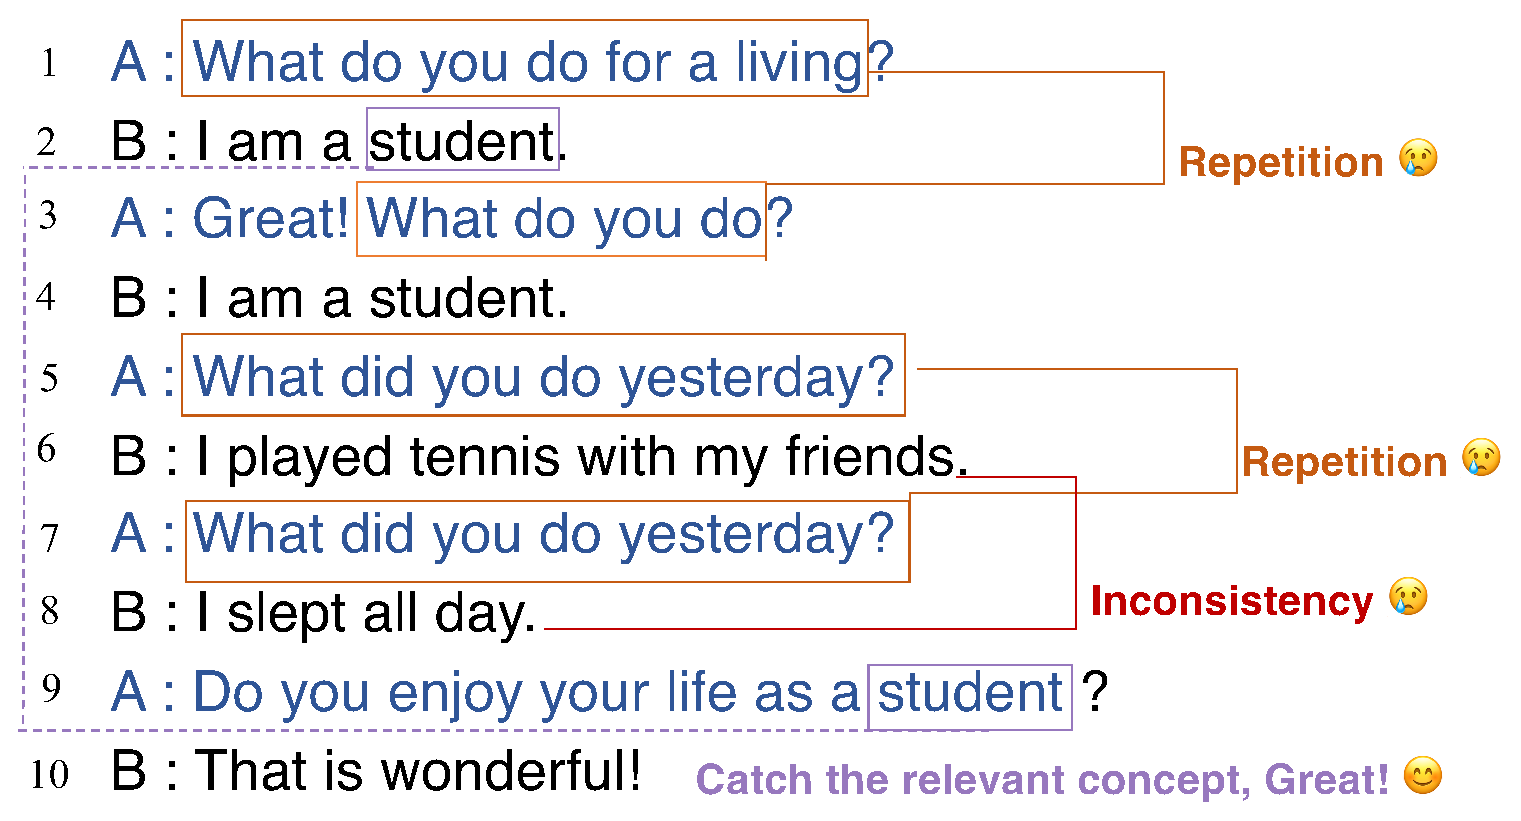
\includegraphics[width=0.95\columnwidth]{example2.eps}
        \caption{A chat snippet between two bots.}
        \label{fig:example}
\end{figure}

Fluency, Knowledge, Proactivity and Specificity are scored for each turn separately
and aggregated at the end of the conversation.
Detection for diversity, consistency and relevance are more involved and are explained
using \figref{fig:example}. 

As for diversity, at each turn $t$, we first check if there exists any repetitive question.  
We can easily find turn 3 and turn 7 repeated turn 1 and turn 5 
respectively. They will then be penalized one point for repetition. 
Repetition is not penalized if the previous turn is already 
marked as a repetitive question. For example, in \figref{fig:example}, 
although turn 4 is considered a repetition of turn 2,  
we are not going to penalize it as turn 3 is a repetitive question. 

The detection of inconsistency is always triggered after the detection of repeated questions. 
If the answers to the same questions are different, we will penalize the current turn, 
such as turn 8 in \figref{fig:example}.

We decide a repetition or an inconsistency by calculating the similarity of the two turns. 
We use a similarity function to complete the calculations, which we will 
discuss in \secref{sec:experiment}. The actual diversity and consistency scores
are the negation from the amount of repetition and inconsistency.

Relevance is assessed as a bonus to reward
a bot if it is able to memorize the important relevant concepts that have shown up 
before in the conversation. We sort the concepts that have shown up in 
chat history by their IDF scores. For example, in turn 9, $A$ 
mentions the concept word ``student'' presented by $B$ in turn 2. With this
turn, $A$ will win a bonus point.


The algorithms and notations for computing diviersty, consistency and relevance are included
in \tabref{tab:functions}, \algoref{algo:rep}, \algoref{algo:inconsist}, and \algoref{algo:bonus}. 

\begin{table}[th]
\centering
\small
\begin{tabular}{c|l}
%\hline
\toprule
\textbf{Notation} & \textbf{Description} \\ \midrule
$t$ & Current turn \\
$H(t)$  &  a list of history turns prior to $t$ \\
$Sim(x,y)$ & similarity between two turns $x$ and $y$ \\
$\sigma_r$ & Threshold for detecting repetition \\
$\sigma_c$ & Threshold for detecting consistency \\
$r$ & Weight for repetition \\
$c$ & Weight for inconsistency \\
$b$ & Weight for bonus \\
$d$ & Min distance between consecutive mentions \\
IDF list & List of lemma in chatlog sorted by IDF\\
$p$ & Percentage of important lemmas in IDF list\\
$R(t)$ &  Repetition penalty for turn $t$ \\
$C(t)$ &  Inconsistency penalty for turn $t$ \\ 
$B(t)$ &  Memory bonus for turn $t$ \\
$Rep(t)$ & A list of repeated turns for turn $t$ \\  
\bottomrule
\end{tabular}
\caption{
Functions and variables in algorithms.}
\label{tab:functions}
\end{table}

\begin{algorithm}[th]
\small
\caption{Scoring for Diversity}
\label{algo:rep}
\hspace*{0.02in} {\bf Input:}
 $t$, $H$, $Sim$, $\sigma_{r}$
; \hspace*{0.02in} {\bf Output: } 
 $R$;
\begin{algorithmic}[1]
\State //Starting to detect repetition
\For {$u$ in $H(t)$}
	\If {$Sim(t,u) \geq \sigma_{r}$}
		\State Add $u$ to $Rep(t)$
	\EndIf
\EndFor
    \If{$len(Rep(t))\geq 0$}
        \If{$t$ is a question and We can find a question in $Rep(t)$}
        \State $ R(t) \leftarrow  R(t) + 1$ 
        \Else
        \If {the previous turn of $t$ is not a repetitive question}
        \State $R(t)) \leftarrow R(t) + 1$ 
        \EndIf
        \EndIf
    \EndIf
\end{algorithmic}
\end{algorithm}


\begin{algorithm}[th]
\small
\caption{Scoring for Consistency}
\label{algo:inconsist}
\hspace*{0.02in} {\bf Input:}
$t$, $H$, $Sim$, $\sigma_{c}$
; \hspace*{0.02in} {\bf Output:  } 
 $C$;
\begin{algorithmic}[1]
\State // Inconsistency detection
 \If {previous turn of $p$ is a repetitive question} 
   \If{ the response $res$ to the question repeated by turn $p$ contradicts turn $i$ with $Sim(t, res) \leq \sigma_{c}$ }
    \State $C(t) \leftarrow C(t) + 1$
   \EndIf
  \EndIf
\end{algorithmic}
\end{algorithm}

\begin{algorithm}[th]
\small
\caption{Scoring for Relevance}
\label{algo:bonus}
\hspace*{0.02in} {\bf Input:}
$t$, $p$, $d$
; \hspace*{0.02in} {\bf Output:  } 
$B$;
\begin{algorithmic}[1]
\State // Assessing the ability of catching relevant concepts\\
$B(t) \leftarrow 0$
\For {all tokens $tk$ in current turn $t$}
 \If {$t$ - previous occurrence turn of $tk > d$ and $tk$ in the top $p\%$ of the IDF list of all tokens in the dialogue} 
   \State $B(t) \leftarrow 1$
  \EndIf
 \EndFor
\end{algorithmic}
\end{algorithm}

At the end of each game, each bot gets seven scores, one for each dimension.  
After pairwise comparison on individual dimension, a bot gains one point for win and zero point for a tie or lose.
The final score of each bot is determined by the sum of their individual scores.
%\KZ{Are these scores positive or negative? Comparable between bots?}

\subsubsection*{Match-level Scoring}
%\KZ{Use an equation to compute the final scores?}
One match which consists of two games, each started with a different bot, 
decides winning or losing between two bots.
For match-level scoring, we mimic the scoring rules of soccer tournament. 
For each match, $W$ points for the winner,  
$T$ points for a tie and 
$L$ points for the loser.
The value of $W$, $T$ and $L$ will be discussed in \secref{sec:ablation}. 

%\KZ{At the match level, we need to consider different starting context for the bots? I think we should present a few options for the reader and say that we are limited to these.}

\subsubsection*{Tournament-level Scoring}
%\KZ{Use an equation to compute the final scores?}
We count the points by simply summing up their scores gained in every match. Currently, several bots with the same final rank are tolerated. For future study, it's possible to mimic more detailed rules presented in sports match such as determine their ranking based on their win-loss relationship in the match between them.  
If they are still tied, we could propose an “overtime” for these two bots, one human judge may observe their performance and then make the decision of the game.

\section{Implementation Details}
\label{sec:imp}

To build the CRF model of Title Classifier, we used a training data
set with 4000 positive and 2000 negative samples.
In this data set, all negative and 50\% of positive samples are real
web page titles from a fragment of Bing snapshot $T_{1}$,
while the remaining samples are synthesized (see \ref{sec:titleDataSet}).
To generate POS tags and lemma features,
we used the \emph{Stanford Part-Of-Speech Tagger}~\cite{toutanova2003feature},
which is a maximum-entropy tagger for English.  % In addition, to optimize the
% accuracy of the tagger, we need to filter ill-formatted writing in the
% title and lowercase all the words before generating the model pattern.

The HTML Parser we use is the Winista HtmlParser \cite{winista}. 
%It is a popular HTML parser written in C\#, and provides very high accuracy
%and efficiency.  
We filter out unwanted lists according to a black list of
tags, including \emph{$<$head$>$, $<$link$>$, $<$style$>$, $<$form$>$,
  $<$iframe$>$, and $<$input$>$}.

For the Top-K Ranker, we propose two approaches, which are labeled as
\emph{rule-based} and \emph{learning-based}, respectively in
Section \ref{sec:eval}.
For the \emph{learning-based} ranker, we build a training set as
follows. \ZZX{First, we use the original system with the
\emph{rule-based} ranker to process web pages from Bing fragment $T_{1}$.}
From the result set, we
select 1000 top-$k$ pages from which top-$k$ lists can be correctly
extracted.  The extracted lists are labeled as positive cases,
while the rest of the candidate lists are labeled as negative ones, 
as our basic assumption is that one top-$k$ page only contains one top-$k$
list.  Then training data set thus contains 1000 positive lists and
2000 negative lists.

As for Content Processor, we use the \emph{Stanford Named Entity
Recognizer}~\cite{finkel2005incorporating} to detect date and
location entities.  The recognizer uses a CRF sequence model,
together with well-engineered features for Named Entity Recognition
in English. 
%Both \emph{Stanford Named Entity Recognizer} and 
%\emph{Stanford Part-Of-Speech Tagger} are components of 
%\emph{Stanford CoreNLP}, a state-of-art toolkit for general NLP tasks.

\section{Experiment}
In this section, we experiment on different NLG tasks. We first present the experimental setup on different tasks. Then, we show the quantitative and qualitative results together with comprehensive analysis and ablation studies.

\subsection{Implementation Details}
We evaluate the newly proposed ICL strategy on five commonly-researched natural language generation tasks: reading comprehension, dialogue summarization, style transfer, question generation and news summarization. Details on the task description, the strong baseline, corresponding  dataset, evaluation metrics and key hyper-parameters for each task are presented as follows.

\begin{table*}[th]
	\scriptsize
	\centering
	\begin{tabular}{lp{1.1cm}rrrcccc}
		\hline
		Task & Dataset & \#Train & \#Val & \#Test & Input & Output & Avg & Std\\
		\hline
		Reading Comprehension & DREAM & 6,116 & 2,040 & 2,041 & ``Q:''+ question + dialogue & answer & 5.59 & 2.61\\
		Dialogue Summarization & SAMSum & 14,732 & 818 & 819 & dialogue & summary  & 24.99 & 13.06\\
		Style Transfer & Shakespeare & 36,790 & 2,436 & 2,924 & original/modern  & modern/original  & 11.63 & 8.19 \\
		Question Generation & SQuAD1.1 & 75,722 & 10,570 & 11,877 & passage + [SEP] + answer & question & 13.09 & 4.27 \\
		News Summarization & CNNDM & 287,227& 13,368& 11,490 & document & summary & 70.97 & 29.59\\ 
		\hline
	\end{tabular}
	\caption{A summary of tasks and datasets. \#Train, \#Val and \#Test refers to the number of samples in the corresponding dataset. Avg and Std are the statistics for the number of output tokens. ``+'' refers to the concatenation operation.}
	\label{tab:taskdata}
\end{table*}

\textbf{Reading comprehension} is the task that answering questions about a piece of text. We use the DREAM dataset~\cite{sun2019dream} where questions are about corresponding dialogues and the answer is a complete sentence in natural language. We neglect the negative choices in the original dataset and formulate it as a NLG task. We adopt the pre-trained language model BART~\cite{lewis2020bart} as the baseline, where the input is a concatenation of a question and the corresponding dialogue made up of speakers and utterances. 
We experiment with  transformers\footnote{\url{https://github.com/huggingface/transformers}} based on the publically available ``facebook/bart-large'' checkpoint \footnote{\url{https://huggingface.co/facebook/bart-large}}.
%The preceding BART model is also adopted as the baseline, whereas the input is a concatenation of question and a dialogue.
The generated answers are evaluated by BLEU scores\footnote{The BLEU-1/2/3/4 scores are computed according the Google's implementation(\url{https://github.com/tensorflow/nmt/blob/master/nmt/scripts/bleu.py}).}~\cite{papineni2002bleu} widely used for QA systems, together with Meteor and Rouge-L F1 as mentioned above. The parameters are also the same as dialogue summarization, except that the early-stop is activated if there is no improvement on the perplexity of the validation set. 


\textbf{Dialogue summarization} is to generate a concise summary covering the salient information in the input dialogue. The preceding model BART has shown to be a strong baseline for this task, where only the dialogue is concatenated into a single sequence as the input. We experiment with  %transformers\footnote{\url{https://github.com/huggingface/transformers}} based on the publically available ``facebook/bart-large'' checkpoint \footnote{\url{https://huggingface.co/facebook/bart-large}} and 
SAMSum dataset\footnote{\url{https://arxiv.org/src/1911.12237v2/anc/corpus.7z}}~\cite{gliwa2019samsum} for daily-chat dialogues. 
The generated summaries are evaluated by comparing with the reference through evaluation metrics, including Rouge-1/2/L F1 scores\footnote{\url{https://github.com/pltrdy/files2rouge}}~\cite{lin2004rouge}, Meteor~\cite{banerjee2005meteor} and BertScore F1\footnote{Both Meteor and BertScore are calculated by SummEval(\url{https://github.com/Yale-LILY/SummEval}), and the latter one is based on the default bert-base-uncased model.}. We evaluate the model on the validation set after each training epoch and the early-stop patience will be added 1 if there is no improvement according to the Rouge-2 F1 score. The training process terminates when the early-stop patience equals or is larger than 3.  During the inference, the minimum and maximum output length is set to 5 and 100 respectively, with no\_repeat\_ngram\_size=3, length\_penalty=1.0 and num\_beams=4.


% The answer is either a span of words in the original text or a complete sentence in natural language.
\textbf{Style transfer} preserves the semantic meaning of a given sentence while modifies it's style, such as positive to negative, formal to informal, etc.
We adopt the Shakespeare author imitation dataset~\cite{xu2012paraphrasing}, containing William Shakespeare's original plays and corresponding modernized versions. Krishna el al.~\shortcite{krishna2020reformulating} proposed to do unsupervised style transfer by training paraphrase models based on the GPT-2 language model~\cite{radford2019language}. We re-implemented their approach STRAT\footnote{\url{https://github.com/martiansideofthemoon/style-transfer-paraphrase}} and evaluated with the provided script. Evaluation metrics includes 
transfer accuracy(ACC), semantic similarity(SIM), Fluency(FL) and two aggregation metrics, i.e., geometric averaging(GM) and their newly introduced $J(\cdot)$ metric. The hyper-parameter $hp$ equaling 0.0, 0.6 or 0.9  in Table~\ref{tab:end2endst} is the sampling parameter for trades off between ACC and SIM in their approach. 
In the training stage, we evaluate the model after updating every 500 steps. The perplexity on the validation set is used to activate the early-stop which equals 3. The inference is done as default.
 
\textbf{Question generation}~\cite{zhou2017neural} aims at generating a question given an input document and its corresponding answer span. SQuAD 1.1~\cite{rajpurkar2016squad} is generally used for evaluation. We adopt the data split as in \cite{du2017learning} and fine-tune the pre-trained UniLM~\cite{dong2019unified} as the strong baseline according to their official implementation\footnote{\url{https://github.com/microsoft/unilm/tree/master/unilm-v1}}. Generated questions are evaluated by metrics including BLEU-1/2/3/4, Meteor and Rouge-L with the provided scripts. The model is evaluated every 1000 steps and the early-stop equaling 3 is associated with the perplexity on the validation set. Other parameters are unchanged following the official guideline.

\textbf{News summarization} differs from dialogue summarization where the input is a document instead of a dialogue. We adopt the same strong baseline BART and evaluation metrics as dialogue summarization. Experiments are done with CNNDM dataset~\cite{HermannKGEKSB15} consisting of news articles and multi-sentence summaries\footnote{\url{https://github.com/pytorch/fairseq/blob/main/examples/bart/README.summarization.md}}. The model is evaluated every 2000 steps and the early-stop equaling 3 is associated with the Rouge-2 on the validation set. During the inference, the minimum and maximum output length is set to 45 and 140 respectively, with no\_repeat\_ngram\_size=3, length\_penalty=2.0 and num\_beams=4.
%\footnote{Inference parameters are borrowed from \url{https://github.com/pytorch/fairseq/blob/main/examples/bart/summarize.py}}

The summary of each task is listed in Table~\ref{tab:taskdata}. For fair comparisons, we re-implemented baselines following the above instructions on our machine. On top of the above baselines, we further arm them with the ICL strategy according to the Algorithm~\ref{alg:picl}. The settings of newly introduce Start and Stride are specified and discussed in following sub-sections. All of our experiments are done on a single RTX 3090 or a single RTX 2080Ti with 24G and 11G GPU memory respectively.
%and the result are averaged over three runs.


 
\subsection{Automatic Evaluations on Different Tasks}
\label{sec:taskperformances}

We compare our approach with the vanilla models mentioned above and the approach from~\citet{liang-etal-2021-token-wise} as baselines.
The performances on different NLG tasks are shown in Table~\ref{tab:end2end}. 
These tasks not only focus on solving different problems, but also has various amount of training data as well
as reference output lengths as shown
Table~\ref{tab:taskdata}.
Besides, the basic model are also different, including BART, GPT-2 and UniLM. 
Our new training strategy achieves significantly improvements among different tasks on most evaluation metrics, which shows that our method not only works well, but also has strong generalization abilities.

We explain the some specific results as follows:

(1) Our training strategy boosts the performances of the original STRAT with different $hp$ in the style transfer task. GM and J are two comprehensive evaluation metrics, with our approach topping the ranks with significant improvements.

(2) TCL generally performs poorly on tasks
with more training data. For example, it failed on question generation without any improvements over the vanilla model under the same parameter setting, while ICL still 
logs gains. This is mainly due to two reasons.
First, because the nature of TCL is data augmentation which is more effective in low-resource settings,
when training data is abundant, it becomes less useful. 
Second, the way they calculate the loss as sub-sequence generation better suites paraphrasing tasks, such as machine translation tested in their paper, as the order of 
the corresponding tokens between input and output 
are almost the same. Learning such forward mapping can 
be regarded as a kind of ``easy-to-hard'' 
in these limited scenarios.
However, this doesn't hold true for other tasks, 
such as summarization and question generation. 
Therefore, we didn't further test it on CNNDM since
CNNDM has the large amount of training data among
the five.

(3) For news summarization, Rouge-1 scores (precision, recall) for the baseline and our method on CNNDM are (38.16, 52.72) and (40.84, 49.23) correspondingly. Our method made substantial improvements on the precision with a compromise on the recall. 
The meteor score based on the unigram precision and recall emphasizes more on the recall than the Rouge-1 F1. As a result, it drops while Rouge-1 F1 increases. Overall, our method still outperforms BART on this task, especially on F1 scores of Rouge-2 and Rouge-L.




\begin{table}[th]
	\small
	\centering
	\begin{subtable}{\linewidth}
		\scriptsize
		\centering
		\begin{tabular}{lcccccc}
			\hline
			{Method} & {B1} & {B2} & {B3} & {B4} & {Met} & {RL}\\
			\hline
			w/o CL &  32.03 & 16.01 & 8.77 & \textbf{4.80} & 19.84 & 38.89\\
			TCL & 32.53 & 16.25 & 8.52 &4.67 &19.88 & 39.65 \\
			ICL &  \underline{\textbf{33.99}} & \underline{\textbf{17.43}} & \underline{\textbf{9.18 }}& 4.64 & \textbf{20.60} & \textbf{40.78}\\

			\hline
		\end{tabular}
		\caption{Reading Comprehension}
		\label{tab:end2endrc}
	\end{subtable}
	\\[5pt]
	\begin{subtable}{\linewidth}
		\scriptsize
		\centering
		\begin{tabular}{lccccc}
			\hline
			{Method} & {R1} & {R2} & {RL} & {Met} & {BertS} \\
			\hline
			%BART & 52.60&27.00 &42.10 &- & - \\
			w/o CL & 51.88 & 27.30 & 42.77 & 24.75 & 71.38 \\
			TCL  & 52.33 & 27.80 & \textbf{43.91} & 24.59 & 71.77 \\
			ICL & \underline{\textbf{53.07}} & \underline{\textbf{28.23}} & {43.83} & \underline{\textbf{26.12}}& \underline{\textbf{72.17}} \\
			
			\hline
		\end{tabular}
		\caption{Dialogue Summarization}
		\label{tab:end2endds}
	\end{subtable}
	\\[5pt]
	\begin{subtable}{\linewidth}
		\scriptsize
		\centering
		\begin{tabular}{lcccccc}
			
			\hline
			{Method}&$hp$ &  {ACC} & {SIM} & {FL} & {GM} & {J}\\
			\hline
			%\multirow{3}{*}{STRAT}& 0.0 & 71.70 & \textbf{56.40} & 85.20 & 70.10 & 34.70 \\
			%& 0.6 & 75.70 & 53.70 & 82.70 & 69.50 & 33.50 \\
			%& 0.9 & 79.80 & 47.60 & 71.70 & 64.80 & 27.50 \\
			%\hline
			\multirow{3}{*}{w/o CL}& 0.0 & 70.49 & 55.70 & 85.98 & 69.63& 33.72 \\
			& 0.6 &75.31 & 53.46 & 82.56 & 69.27& 33.30\\
			& 0.9 & 78.76 & 47.38 & 74.42 &65.24 & 27.88\\
						\hline
			\multirow{3}{*}{TCL } & 0.0 & 70.31 & \textbf{55.95} &\textbf{87.24} &  70.01& 34.71 \\
			& 0.6 & 74.79 & 53.14 & 82.56 & 68.97 & 33.21 \\
			& 0.9 & 79.41 & 46.88 & 71.92 &64.45 & 26.92 \\
			\hline
			\multirow{3}{*}{ICL}& 0.0 & \underline{73.72} & 55.91 & 86.30 & \underline{\textbf{70.60}} &\underline{\textbf{35.81}}\\
			& 0.6 & 77.26 & \underline{53.80} & \underline{83.87} & \underline{70.38} & 34.64\\
			& 0.9 & \textbf{79.65} & 48.16 & 76.06 & 66.32 & 29.03\\

			\hline
		\end{tabular}
		\caption{Style Transfer.}
		\label{tab:end2endst}
	\end{subtable}
	\\[5pt]
	\begin{subtable}{\linewidth}
		\scriptsize
		\centering
		\begin{tabular}{lcccccc}
			\hline
			{Method} & {B1} & {B2} & {B3} & {B4} & {Met} & {RL}\\
			\hline
			w/o CL & \textbf{50.38} & 35.67 & 27.24 & 21.36 & 24.40 & 50.67 \\
			TCL &\textbf{50.38} & 35.67 & 27.24 & 21.36 & 24.40 & 50.67\\
			ICL &  50.18 & \textbf{35.72} & \textbf{27.36} & \textbf{21.54} & \textbf{24.57} & \underline{\textbf{51.09}} \\
			\hline
		\end{tabular}
		\caption{Question Generation}
		\label{tab:end2endqg}
	\end{subtable}
		\\[5pt]
	\begin{subtable}{\linewidth}
		\scriptsize
		\centering
		\begin{tabular}{lccccc}
			\hline
			{Method} & {R1} & {R2} & {RL} & {Met} & {BertS}\\
			\hline
			%BART &  \\
			w/o CL &  43.07 & 20.01 & 35.94 & \textbf{21.44} & 63.72 \\
			TCL & - & -&- &- &- \\
			ICL & \textbf{43.39} & \underline{\textbf{20.55}} & \underline{\textbf{36.63}} & 19.68 & \textbf{64.05}\\
			\hline
		\end{tabular}
		\caption{News Summarization}
		\label{tab:end2endns}
	\end{subtable}
	\caption{Performances on different NLG tasks. ICL represents the models trained with our ICL algorithm. TCL refers to the previous work from~\cite{liang-etal-2021-token-wise}. Scores underlined are statistically significantly better than both re-implemented baselines with $p<0.05$ according to t-test. }	
	\label{tab:end2end}
\end{table}


\subsection{Human Evaluations}

To further prove the improvement of ICL, we hired three proficient English speakers for human evaluation. 20 samples from the test set of each task are randomly selected, ignoring the ones with totally same generations among three models, including the vanilla model, TCL and ICL. The original input, reference output and three generations are shown to annotators together, while the order of three generations are unknown and different among samples. 3-point Likert Scale is adopted for scoring for each generation~\cite{gliwa2019samsum}, where [1, 3, 5] represent 
excellent, moderate and disappointing results 
respectively. The average scores and agreements 
among the annotators are shown in 
Table~\ref{tab:humaneval}.

The Fleiss Kappa on the first four tasks indicates the fair to moderate agreements. It shows the promising improvement of ICL over the vanilla model and TCL especially on DREAM, SAMSum, and SQuAD1.1, which is consistent with the conclusion based on automatic metrics.
Although the agreement on style transfer is fair, 
our annotators without Shakespeare background 
tend to give low scores to all outputs.
Therefore, the absolute improvement is 
only $0.04$ compared to both baselines.
%This mainly due to the indistinguishable styles between
%Shakespeare’s plays with are quite different from modern languages. 
Besides, the poor agreement on CNNDM reflects the 
diverse concerns of summarization from different 
annotators. Without more specific instructions, they 
tends to focus more on the content coverage instead 
of checking the detailed facts. This is also 
consistent with the higher Meteor scores of the 
vanilla model over ICL.

\begin{table}[th]
	\scriptsize
	\centering
	\begin{tabular}{l|ccc|c}
		\hline
		{Datasets} & {w/o CL} & {TCL} & {ICL} & {Agreement}  \\
		\hline
		DREAM  &3.07 & 2.50&3.20 &0.48 \\
		SAMSum &2.97 &3.57 &3.97 &0.40 \\
		Shakespeare &2.23 &2.23 & 2.27&0.32 \\
		SQuAD1.1 &3.43 & 3.43 &3.77 &0.35 \\
		CNNDM & 3.45 &- &3.40 &0.11 \\
	%	\hline
	%	overall & & & &\\
		\hline
	\end{tabular}
	\caption{Human evaluations. The agreement is calculated by Fleiss Kappa.}
	\label{tab:humaneval}
\end{table}




%Following Liu et al.\shortcite{liu2021competence}'s work, we asked annotators to comparing the performance between our generated results and baselines by choosing from ``Better, Tie, Worse''. 
%The counts for each choice are shown in Table~\cite{}, where the Fleiss Kappa among annotators is ??.

%Analysis





%\subsection{Analysis on Variable Generation Lengths}

%Teacher forcing, which predicts each token given the reference summary tokens during training and given the previous generated tokens during inference, leads to the exposure bias problem for NLG tasks.
%Since ICL starts the training process by predicting the last few tokens of outputs and gradually calculates the loss based on more tokens when the model is stronger, we hypothesis that it can alleviate the exposure bias for training Seq2Seq models to some extent.
%As stated in~\cite{pang2020text}, the output quality tends to degrade as the output length increase with the exposure bias.
%So, we divided the test set of each task according to the length of the generated output into 4 buckets and randomly picked 20 samples in each buckets for both the corresponding baselines and our approach. Each generation is annotated by 5 point Likert Scale, where 1 is the worst and 5 is the best. 

%The trends of performances on variable generation lengths are in Figure~\ref{}.


\section{Related Work}
\label{sec:related}
The top-$k$ list extraction problem, presented in this work,
belongs to the general area of web structured data extraction,
where many techniques have been developed and improved recently.
In general, these techniques can be categorized as follows:
(a) heuristic methods \cite{googlesets,webtables08};
(b) automatic extraction rule discovery \cite{ChangL01:IEPAD};
(c) similarity-based extraction \cite{LiuGZ03:MDR,MiaoTHSM09:TagPathClustering}; and
(d) visual model and features \cite{GatterbauerBHKP2007:Towards, FumarolaWBMH11:List}.

Google Sets \cite{googlesets} and WebTables \cite{webtables08}
extract web lists or tables based
on very specific list-related tags, such as {\tt <UL>},
{\tt<OL>}, {\tt<DL>}, and {\tt<TABLE>}.
IEPAD \cite{ChangL01:IEPAD}
identifies repetitive substrings as list patterns
in an encoded document/web page.
MDR \cite{LiuGZ03:MDR} is proposed to extract data records of the same type
based on the similarity between DOM trees, which is measured by edit distance.
Miao et al. \cite{MiaoTHSM09:TagPathClustering} introduce the visual signal
which is a vector describing tag path occurrence patterns.
Based on a similarity measure between visual signals, they perform clustering of tag
paths and rebuild the structure of data in the form of sets of tag paths.
Ventex \cite{GatterbauerBHKP2007:Towards} uses CSS2 visual box
model \cite{CCS2Box} instead of DOM trees to represent web pages,
and extract web tables based on several rules and heuristics.
HyLiEn \cite{FumarolaWBMH11:List} is a hybrid list extraction approach
as it not only utilizes the visual alignment of list items
but also takes advantage of structural feature (DOM tree).
And it claims a remarkable improvement compared with Ventex\cite{GatterbauerBHKP2007:Towards}.

In general,  category (c) and (d) are more practical,
as the (a) and (b) are not very robust against evolving or complicated web pages.
(d) often has better accuracy since web pages are rendered for visual presentations,
thus the visual models should be more expressive
and intuitive in representing a list or table.
Nevertheless, (c) is often more efficient in time as it does not need to render the page.

Although our system is inspired by some of approaches above
(e.g, we improve tag path clustering by Miao et al. \cite{MiaoTHSM09:TagPathClustering}
and use it in list extraction), it has several major differences:
%most of them cannot effectively address the top-$k$ extraction problem
%for several reasons:
\begin{itemize}
  \item \emph{Different goals}:
  The goal of previous approaches is to indiscriminatingly extract all lists
  or tables from a web page, while ours is to extract one specific list from a special
  kind of page while purging all other lists.
  \item \emph{The use of number $k$}:
  Our method takes advantage of the top-$k$ list size $k$,
  which is inferred from title. This is important to filter most of noise lists.
  \item \emph{Understanding semantics}:
  We understand each top-$k$ list as a list of instances with attributes
  with respect to the concept in the title.
  This is critical not only for identifying the correct list, but also for
  the future application of the extracted results.
  \item \emph{Time Efficiency}:
  On average, our system can process a page in about 0.1 second,
  which is significantly faster than the previous approaches 
  (Miao\cite{MiaoTHSM09:TagPathClustering}: $\approx 0.3s$;
  HyLiEn\cite{FumarolaWBMH11:List}: $4.2s$).
  This is key to scaling up the system to process billions of pages.
\end{itemize}

We first introduced the concept of ``top-$k$'' list
in a demo paper \cite{ZZX2012KDD}.
In that demo, we proposed the top-$k$ list extraction problem
and designed a prototype system.
We presented this prototype as a web GUI
on the project website \cite{list-extractor}.

One of the potential use of the extracted top-$k$ lists
is to act as background knowledge for a Q/A system\cite{cao2012approaches} to answer
top-$k$ related queries. To prepare for such knowledge, we need techniques
to aggregate a number of similar or related lists into a more comprehensive
one, which is in the space of top-k query processing.
One of the most well-known algorithms there is
TA (threshold algorithm) \cite{fagin2001optimal,guntzer2000optimizing}.
TA utilizes aggregation functions
to combine the scores of objects in different
lists and computes the top-$k$ objects based on the combined score.
Later, Chakrabarti et al. \cite{chakrabarti2006ranking} introduced the
OF (object finder) query,
which ranks top-$k$ objects in a search query
exploring the relationship between TOs (Target Objects, e.g., authors, products)
and SOs (Search Objects, e.g., papers, reviewers).
%OF differs from TA in that each TO can be related to multiple SOs,
%thus an additional aggregation of multiple scores within
%each list is needed.
Bansal et al.\cite{bansal2008ad} utilize a similar framework but
elevate terms at a higher level by taking advantage of a taxonomy,
in order to compute accurate rankings.
Angel et al.\cite{angel2009ranking} considered
the EPF (entity package finder) problem which is concerned with
associations, relations between different type of TOs.
Some of these techniques can serve as the basis for comprehensive integration of
top-$k$ lists.
%The output is a ranked list of a package which is a tuple of different type of objects.

%Unfortunately none of the above approaches can be applied directly to our problem,
%because in the approaches above, SOs (documents or reviews) are treated equally,
%whereas in our problem, lists from different sources (web pages) should be
%weighed differently.
%For example, lists from more popular web sites should be given more weight as
%their content are more trustable.
%In addition, lists that are exactly the same should be count only once
%as they may be reshipments from one source.


%%
% File emnlp14-rumor\paper.tex
%
\documentclass[10pt,final,conference,letterpaper]{IEEEtran}
\usepackage{times}
\usepackage{url}
\usepackage{latexsym}
\usepackage{amsmath,algorithm,algpseudocode,caption,subcaption}
\usepackage{epsfig}
\usepackage{graphicx}
\usepackage{booktabs}
\usepackage{color}
\DeclareCaptionType{copyrightbox}
%\setlength\titlebox{6.5cm}    % Expanding the titlebox
\newcommand{\triple}[3]{$\langle$#1, #2, #3$\rangle$}
\newcommand{\pair}[2]{$\langle$#1, #2$\rangle$}
\newcommand{\figref}[1]{Figure \ref{#1}}
\newcommand{\tabref}[1]{Table \ref{#1}}
\newcommand{\secref}[1]{Section \ref{#1}}
%\newcommand{\eqref}[1]{Eq. (\ref{#1})}
\newcommand{\KZ}[1]{\textcolor{blue}{[Kenny: #1]}}
\newcommand{\WK}[1]{\textcolor{red}{[Ke: #1]}}
\newcommand{\ZY}[1]{\textcolor{red}{[Zhiyi: #1]}}

\begin{document}
\title{ExtRA: Automatic Extraction of Review Aspects 
%\Thanks{}
}

\author{
Shi Feng, Kenny Q. Zhu, Zhiyi Luo\\
%Shi Feng$~^{1}$, Kenny Q. Zhu$~^{2}$, Zhiyi Luo$~^{3}$\\
%\vspace{1.6mm}
\fontsize{10}{10}\selectfont\itshape
%Department of Computer Science \& Engineering\\
Shanghai Jiao Tong University, Shanghai, China\\
\vspace{-1cm}
%\fontsize{9}{9}\selectfont\ttfamily\upshape
%$~^{1}$sjtufs@gmail.com, $~^{2}$kzhu@cs.sjtu.edu.cn, 
%$~^{3}$jessieluo1991@gmail.com
}

%\date{\today}
\maketitle
\begin{abstract}
Summarizing users opinions about a product or
service by rating against several distinct and representative aspects
is intuitive and effective. Manual determination of aspects of a product type 
doesn't scale to large and comprehensive e-commerce or consumer review sites
and doesn't adapt to changes in interests.
This paper demonstrates a unsupervised multistage
approach for automatically discovering the best aspect words from massive
amount of textual user reviews of any type of product or service. 
Our experiments showed that the approach is efficient and achieves 
the state-of-the-art accuracies.
\end{abstract}

\section{Introduction}
\label{sec:intro}

Product reviewing is a key character that distinguishes e-commerce 
from conventional retail.
Many websites provides either qualitative or quantitative
summaries of user reviews, organized by important aspects 
of the target product or service.
One example of such \emph{aspect-based review 
summarization}~\cite{hu2004mining} for a hotel on TripAdvisor
as of June 2016 is shown in \figref{fig:tripadvisor}. 
Here, besides the short review passage written by the user, 
the user are asked to give discrete ratings (on the scale of 1-5) 
on various aspects of the hotel room, 
e.g., location and cleanness. The ratings of 
a product from individual reviews can then be aggregated into an overall
ratings of the same product by many users.

\begin{figure}[th]
\centering
\includegraphics[width=0.7\columnwidth]{figures/tripadvisor-short}
\caption{Part of a user review from TripAdvisor.}
\label{fig:tripadvisor}
\end{figure}


Aspect-based review summaries strike a nice middle ground between
detailed text reviews and an all-in-one overall score, yielding
a somewhat balanced view of a product. Such summaries
provide an effective and efficient way of comparing products in
the same category.
%have several advantages compared to the more traditional 
%style of online reviews that consists of a short passage and 
%an overall rating. 
%In aspect-based reviews, more details are provided quantitatively and 
%more directly, and the users can learn about various aspects of a product 
%without having to read the entire review passage. Another advantage of 
%aspect-based reviews is that different products within the same category 
%can be compared directly with respect to multiple aspects, 
%instead of just an overall rating. When researching on products, 
%users spend most of their time comparing different brands and models. 
%Aspect-based review summarization provides an effective and efficient way for 
%doing such comparison, saving the users both time and effort.


%At present, websites that offer aspect-based review summaries typically 
%only feature a single or a small number of product categories, e.g.,
%TripAdvisor.com only features travel related products while Cars.com reviews
%automobiles. 
Because it takes in-depth knowledge to 
characterize a product type using a few keywords that balance between
relevance and diversity, at present, these aspects are primarily hand picked
by the review site operators.
Manual selection of aspects cannot scale to large number of
product types as featured by general e-commerce platforms such as Amazon.com
and Yelp. Moreover, such aspects may change from time to time due to 
evolving user interests.
%These platforms instead turn to automatic review 
%summarization, mined from the user review texts. 

%\begin{figure}[th]
%\centering
%\includegraphics[width=0.8\columnwidth]{figures/phrases}
%\caption{Automatic review summarization for two mobile phones 
%on an e-commerce website}
%\label{fig:phrases}
%\end{figure}
%
%An example of automatic review summarization commonly seen 
%on e-commerce websites is shown in \figref{fig:phrases}. 
%There is a summary of opinion phrases for each phone model, 
%along with the frequency of each phrase mentioned in the 
%reviews. There are two major drawbacks in this form of summarization. 
%First, it is restricted to using the reviews about a specific product. 
%Therefore, summaries are incompatible across different products within 
%the same category - different models may not share the same set of 
%opinion phrases. This makes it less useful for users to compare
%different models.  Second, users' sentiment toward 
%each aspect cannot be quantified and computationally compared - 
%the difference of emotional strength between 
%``extremely good" and ``above average" is hard to capture.
% user cannot choose to express them differently.

%The aspects of a product are supposed to capture the most important features 
%and cover all the facets of the product. The products of the same category 
%share the same set of aspects, however the aspects can be very different 
%across categories. It takes both common knowledge and personal experience 
%with the product to decide which are the appropriate aspects. 
%The websites that can provide aspect-based rating system basically 
%all share a common feature, that is they each focuses on only one or 
%a small range of products. For example TripAdvisor focuses on hotels and 
%Cars.com focuese on cars. The set of aspects is what the consumers base 
%on to compare different products, thus they must be carefully chosen 
%to cover all the facest of the product. Moreoever, at the end of the day 
%the aspects is designed to serve the consumers, especially potential consumers, 
%so they need to reflect what the consumers care about the product. 
%Ideally, the aspects should be decided with user reviews taken into 
%consideration. For a small range of products, the website owner or 
%the retailer may manual designate the set of aspects, 
%however this is intractable for websites like Amazon and TaoBao, 
%which host basically all kinds of products available on the market, 
%and websites like Yelp on which users review thousands of different services. 
%
%Motivated by this observation, we are in need for methods that automatically 
%generate review summarizations. 

Our goal in this paper is to develop an unsupervised system 
for aspect word extraction from a set of user reviews about products within 
the same category.  This problem is similar to topic modeling where aspects 
can be seen as topics, but with a few differences: 
\begin{itemize}
    \item in aspect extraction, we seek to produce 
	aspect words with small mutual semantic overlap; 
    \item aspects may be expressed implicitly through personal experience; and
    \item reviews are a short piece of text, 
	  hence the topics may shift very quickly from 
          sentence to sentence.
\end{itemize}
Previous unsupervised methods for aspect extraction are 
variations of topic models, and cannot capture word semantics and thus
the implicit reference of product aspects. 
In our method we leverage the distributed 
representations of words and sentences. With distributed representations, 
the semantic similarity between two sentences can be more accurately 
calculated without relying too much on the lexical information.
Our proposed method consists 3 clustering steps and
2 ranking phases. The framework achieved state-of-the-art performance 
in end-to-end aspect extraction across multiple domains.

%In \secref{sec:method} we introduce our method step-by-step.
%In \secref{sec:experiments} 
%we evaluate our method on user reviews from multiple domains and demonstrate 
%the effectiveness of our model against other approaches 
%and show how the aspects extracted can be used
%to construct a complete review summarization. 
%In \secref{sec:related}, we discussed
%and compare our work with previous research on aspect-based review 
%summarization.

\section{The System}
\label{sec:method}

The review aspect extraction problem aims to infer $K$ noun 
words from user reviews about the same product type.
Each word represents a distinct aspect or feature of the product type. 
%Here $K$ is an constant parameter for the problem. 
%In unsupervised models for aspect extraction, 
%the set of reviews and the number of aspects are the only inputs.
%Note that in this definition we don't use cross-domain information, 
%that is, for one product type we only use the reviews of that domain.
%This allows us to apply the model to any domain with ease.
%\begin{figure}[th]
%\centering
%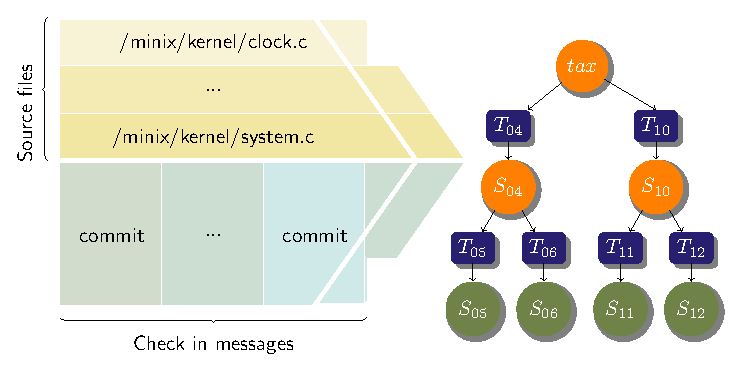
\includegraphics[width=0.9\columnwidth]{figures/framework}
%\caption{Our framework.}
%\label{fig:framework}
%\end{figure}
%
Our system framework consists of 5 steps.
%
%\begin{itemize}
%    \item \textbf{Sentence Clustering}
%
%        We convert each sentence in the reviews into a vector representation 
%        and cluster them in to $N$ clusters of semantically similar sentences.
%
%    \item \textbf{Noise Isolation}
%
%        %As aspects appear as topics in the reviews, 
%        %we use a topic model to infer the potential aspects.
%        To isolate the noises that exist in the sentence cluster,
%	for each sentence cluster we further generate $M$ 
%	topics, resulting in $N\times M$ different word distributions in total.
%
%    \item \textbf{Aspect Inference}
%        
%        We treat each word distribution as a vector and cluster the topics 
%	into $C$ clusters which are the potential aspects. 
%	Here $C$ is purposely set to be larger than $K$. The extra
%	$C-K$ clusters models the redundant aspects.
%        Each cluster contains $N\times M / C$ word distributions, or vectors.
%        We take the mean of these vectors to form $C$ aspect clusters,
%        each being a set of words and their corresponding weights.
%
%    \item \textbf{Cluster Ranking}
%
%        We define a score for the quality of each aspect cluster,
%        and the clusters are ranked by this score.
%
%    \item \textbf{Word Ranking}
%
%        We use WordNet to calculate the semantic distances between the words 
%	in each cluster and adjust the ranking based on the 
%	both the distances and the weights of the words. The top words in each
%	cluster are candidates of the aspect words.
%\end{itemize}
%
%In the following we will explain the motivation and the details of each of
%the five steps. 
%
\subsection{Sentence Clustering}

%One important feature of user reviews is that many topics are 
%compressed into a short paragraph, where each topic corresponds to 
%a potential aspect of the product. 
%A typical hotel review extracted from \figref{fig:tripadvisor} 
%is shown as follows:
%
%\begin{quote}
%Pool is small and only 4 ft but refreshing. Hot tub also there. Staff were super friendly each day. Room was nothing special but clean and comfy. Lots of restaurants and bars nearby. Breakfast was great and despite being a busy weekend there was always a big selection available.
%\end{quote}
%
%In user reviews, topics can shift very quickly.
%Sentences that are close to each other may refer to 
%completely different aspects about the product. Also,
%sentences about the same aspect may not appear in the review consecutively. 
%The existence of such fine-grained semantic shifts in user reviews 
%makes it difficult to apply the the bag-of-word abstraction 
%of normal topic model on reviews.
%Therefore we propose to work on the sentence level instead 
%of the document level, and it would be helpful if we can divide the 
%reviews into topic-oriented segments.
%
%Driven by this observation, in our method the first step is 
%sentence clustering.  For this purpose, 
We represent each sentence in a high-dimensional vector space,
%Instead of using simplistic methods like bag-of-word vector, 
%we leverage a recent development of neural network in natural 
%language processing, the distributed representation.
%In a distributed representation, words and sentences are 
%converted into real-valued vectors.
%The distance of the vectors in the vector space will capture the 
%semantic similarity of the words or sentences.
%In this work we attempt two models, 
using either LSTM (a variant of RNN) or paragraph vector (PV) \cite{le2014distributed}.
%
%\paragraph{Recurrent Neural Network}
%To use RNN for obtaining sentence vectors, 
%we train a neural language model on the review sentences. 
%After the perplexity converges, we use the trained network to 
%process each sentence of the dataset and take the last hidden vector as 
%the vector representation of the sentence. In our method we use a 
%variation of RNN, long-short term memory (LSTM)~\cite{hochreiter1997long} 
%which is reported to have better performance at 
%modeling long sentences \cite{jozefowicz2015empirical}.
%
%\paragraph{Paragraph Vector}
%PV is a simple but powerful extension to Word2vec \cite{mikolov2013distributed} with two components, 
%distributed memory (PV-DM) and distributed bag-of-word (PV-DBOW). 
%The first one is similar to skip-gram in Word2vec and 
%the second is similar to CBOW \cite{mikolov2013distributed}.
%An important advantage of paragraph vector models is that they require 
%no labeled data. Also, it doesn't require human experts to assign weights 
%for words in a paragraph based on linguistic knowledge. 
%The learned vector representations inherit an important property of Word2vec, 
%that is the semantics similarity. Also the final paragraph vector captures the 
%word order information with the part learned from PV-DBOW with the n-gram model.
An advantage of paragraph vector over RNNs is that it can 
leverage trained word vectors, thus requires a smaller training data set. 
%The word vectors can be trained on 
%a much larger corpus so they capture the semantics relationships more 
%accurately.  Consequently, the paragraph vectors can be trained on 
%a relatively small dataset. 
%The performance of paragraph vectors can also be boosted by using pre-trained 
%word vectors that are trained on a larger dataset \cite{mikolov2013linguistic}. 
%%However, previous research show that it is more suitable 
%%to train the word vectors simultaneously for RNNs, 
%%so RNNs cannot leverage the word vectors learned from a larger dataset. 
%Also, the paragraph vector models are simple and 
%don't require the storage of a lot of information. In contrast, for RNN we 
%need to store every state during the forward pass for back-propagation, 
%which is very memory consuming.
%\paragraph{Clustering Sentence Vectors}
We run k-means clustering on the sentence vectors and generate 
$N$ sentence clusters. We then collect the sentences from the same review 
that are clustered together to form smaller fragments of reviews. 
Each original review is divided into several smaller review fragments, 
each belonging to one of the $N$ clusters. As a result, we obtain $N$ 
clusters of review fragments. 

\subsection{Noise Isolation}
There exists noises and overlaps in the clusters formed above.
%The first step, sentence clustering, we might include noise and the sentences 
%within a cluster might not all be about the same aspect. 
%The reason is due to the common occurrences of sentences such as the following
%in the reviews (taken from TripAdvisor):
%
%\begin{quote}
%The room was clean, the staff were friendly, and I would say the price is very reasonable given the proximity to business and leisure destinations around downtown.
%\end{quote}
%
%\begin{quote}
%There is a restaurant just 5 min walk away with nice italian food, pizza was great.
%\end{quote}
%
%In the first sentence multiple aspects are mentioned; in the second sentence, the only aspect is location however lexically it seems to be talking about food.
%With these complicated structures within, 
%it is difficult for RNN or PV to correctly determine the aspects 
%in these sentences. The result is overlaps between clusters about 
%different aspects and noises within each cluster.
%To isolate the noises and resolve such overlap, 
We fix that by applying LDA topic modeling within each sentence cluster, 
treating each review fragment as a document, and generating $M$ smaller topics. 
This will give us in total $N\times M$ topics, or, word distributions. 
%\tabref{table:overlap} shows an example of topics inferred from three
%sentence clusters from hotel reviews and illustrates the overlap problem.
%In this example, five topics were extracted from each sentence cluster, 
%and each row is one topic. It can be seen that the aspects for the 
%three clusters should be {\em room}, {\em location} and {\em price} 
%respectively.
%However, topics shown in boldface font obviously belong to 
%other clusters.  Especially, the last topic of the third cluster 
%appears to be an overlap of more than two clusters.
%The noise isolation step effectively separates the noise topics from other
%topics semantically corehent within a sentence cluster.
%
%\begin{table}[th]
%\centering
%\caption{Topics extracted from three sentence clusters of hotel review.}
%\label{table:overlap}
%\begin{tabular}{|c|l|}
%\hline
%& room bed bedroom size floor \\
%Sentence
%& bedroom room wall size decor \\
%cluster 1
%& room bathroom shower water towel \\
%& room suite size view floor \\
%& room shower area kitchen bed \\\hline
%
%& station minute tube location bus \\
%Sentence
%& location price night place rate\\
%cluster 2
%& location square station street subway\\
%& distance bus subway downtown shopping\\
%& \textbf{restaurant} \textbf{city} \textbf{food} \textbf{buffet} \textbf{place} \\\hline
%
%& price rate service money star\\
%Sentence
%& \textbf{location} \textbf{city} \textbf{star} \textbf{time} \textbf{rate} \\
%cluster 3
%& price service night money city\\
%& price location place night city\\
%& \textbf{location} \textbf{service} \textbf{food} \textbf{price} \textbf{restaurant} \\\hline
%\end{tabular}
%\end{table}


\subsection{Aspect Inference}
\label{sec:topic_clustering}
Each topic is a word distribution, represented by a vector. 
We obtain  more compact representations of those topics by using PCA to 
reduce the topic vectors to 100-dimension.
%We use PCA to reduce the topics vectors to 100-dimension by  
%selecting the 100 words that best distinguish different topics.
Then we perform k-means clustering on the $N\times M$ topics vectors to 
generate $C$ clusters, each containing $(N\times M)/C$ topics.
These are called {\em aspect clusters}.
We set $C$ to be slightly larger than the desired number of product 
aspects $K$, so that the noisy topics can be clustered together and 
later discarded. 
%In an experiment we will evaluate the influence of this redundant clusters on 
%the quality of the final aspects.
%
%\begin{table}[th]
%\caption{Aspect clusters extracted from hotel reviews.
%Each row shows the candidate words of an aspect, sorted by the weight of each word.}
%\label{table:step3}
%\centering
%\begin{tabular}{|l|} \hline
%breakfast, meal, food, tasty, dinner, morning, coffee, tea \\\hline
%room, night, time, bed, day, bathroom, staff, area, place \\\hline
%staff, desk, service, friendly, reception, concierge, helpful \\\hline
%close, city, location, place, central, station, bus, street\\\hline
%bed, shower, spacious, room, size, bathroom, bedroom, floor \\\hline
%price, room, check, night, money, city, location, star, service \\\hline
%location, price, room, night, place, rate, money, time, city  \\\hline
%\end{tabular}
%\end{table}
%
%Finally, for each cluster we take the mean of the $(N\times M)/C$ 
%topics and normalize it
%for the word distribution of that cluster.
%Some example aspect clusters extracted from hotel reviews are 
%shown in \tabref{table:step3}.

\subsection{Cluster Ranking}

We rank the clusters by how ``distinct'' each cluster is from other clusters. 
If a cluster is similar to other clusters, it is considered redundant and of
low quality. We discard $C-K$ least distinct clusters.


%For the $i$th cluster $C_i$ ($i\in [1, C]$), 
%the distinctiveness score $S(i)$ is defined by:
%
%\begin{align}
%S(i) &= \sum_{w\in C_i} S_i(w) \nonumber\\ 
%     &= \sum_{w\in C_i} \log\left(\frac{f_i(w)}{\sum_{j\neq i} f_j(w)}\right)\nonumber \\
%     &= \sum_{w\in C_i}\left[\log f_i(w) - \log\sum_{j\neq c} f_j(a)\right]
%\end{align}
%
%\begin{table}[t]
%\caption{Aspect clusters ranked by distinctiveness score.
%Potential aspect words are boldfaced.}
%\label{table:clustersranked}
%\centering
%\begin{tabular}{|l|} \hline
%\textbf{staff}, desk, \textbf{service}, friendly, reception, concierge, helpful \\\hline
%breakfast, meal, \textbf{food}, tasty, dinner, morning, coffee, tea \\\hline
%\textbf{price}, room, check, night, money, city, location, star, service \\\hline
%bed, shower, spacious, \textbf{room}, size, bathroom, bedroom, floor \\\hline
%close, city, \textbf{location}, place, central, station, bus, street \\\hline
%\textcolor{red}{room, night, time, bed, day, bathroom, staff, area, place} \\\hline
%\textcolor{red}{location, price, room, night, place, rate, money, time, city} \\\hline
%\end{tabular}
%\end{table}
%
\subsection{Word Ranking}
\label{sec:word_ranking}

We rank the words in each cluster 
by considering two factors (similar to TF-IDF): 
the representativeness of the word to the host
cluster; the number of times the word appears in other clusters. 
The most representative word in each cluster
is assumed to be the closest to the centroid of the word cluster.
The distance between two words is the inverse of 
cosine similarity between the word2vec
vectors of the two words.
Then we process the clusters in the order of 
the cluster ranking given in the last step.
When we calculate the score for word $x$ cluster $C_i$,
we also consider the scores of word $x$ in clusters $C_1$ to $C_{i-1}$, 
where the scores have already been calculated. 
We prevent the duplicate aspect words by subtracting the scores 
of $C_1$ to $C_{i-1}$, from the score of $C_i$.
%The score of word $x$ in the $i$th cluster $C_i$ is thus defined by:
%
%\begin{equation}
%s_i(x) = u_i(x) \sum_{y\in C_i}\hat{x}\cdot \hat{y} - \sum_{j=1}^{i-1}s_j(x),
%\label{eq:wordscore}
%\end{equation}
%where $\hat{x}$ is the vector representation of x; $u_i(x)$ is the weight of $x$ in cluster $C_i$.
The words in each cluster is thus ranked by this final score.

\section{Evaluation}
\label{sec:experiments}

We evaluated our framework
against a number of baselines including the state-of-the-art approaches.
%in the end-to-end aspect extraction task.
Our dataset is reviews for 15 categories of product or service crawled from
e-commerce sites such as Amazon.com and Yelp. 
%The review content is plain English text and we do not use any labels 
%for training our model. We use human labels for evaluation. 
%The product categories, their sources and the sizes of the review datasets
%are summarized in \tabref{table:dataset}
%
%\begin{table}[th]
%\centering
%\caption{Dataset summary.} 
%\label{table:dataset}
%\begin{tabular}{|c|c|r|r|}
%\hline
%Product type & Source & No. of Reviews & No. of Words \\ \hline \hline
%hotel        & TripAdvisor & 27145   & 210 \\\hline
%mobile phone & Amazon & 3716    & 136 \\\hline
%mp3 player   & Amazon & 2745    & 128 \\\hline
%laptop       & Amazon & 5471    & 97  \\\hline
%tv           & Amazon & 1237    & 102 \\\hline
%shoes        & Amazon &1748    & 82  \\\hline
%headphone    & Amazon & 1647    & 122 \\\hline
%gps          & Amazon & 1726    & 72  \\\hline
%transportation & Yelp & 3077  & 131 \\\hline
%restaurant   & Yelp & 4016    & 176 \\\hline
%gym          & Yelp & 2481    & 230 \\\hline
%shopping     & Yelp & 2718    & 123 \\\hline
%car dealer   & Yelp & 2839    & 190 \\\hline 
%movie        & Pang et al. \cite{pang2002thumbs} & 3000    & 194 \\\hline
%car          & Cars.com & 1074    & 147 \\\hline
%\end{tabular}
%\end{table}
%
%
%For evaluation, we ask 5 college students proficient with English 
%to annotate ground truth
%aspect words for each product category. For each category, 
%we ask them to provide 5 different words that cover the most important 
%aspects of the corresponding product or service. The labels provided by the
%5 annotators are aggregated together without removing duplicated words, 
%so we have 25 words in total. 
%When evaluating the models, 
%we compare the 5 aspect words generated by the models with those provided 
%by the annotators. 
%We calculate the portion of words among the 25 labels that 
%are correctly generated by the model as the accuracy of the model.
%The ground-truth labels for two product categories are shown 
%in \tabref{table:labels}.
%
%
%\begin{table}[th]
%\centering
%\caption{Labels for hotel and shopping. Each row is provided by one annotator.}
%\label{table:labels}
%\begin{tabular}{|c|l|}
%\hline
%\multirow{5}{*}{hotel}
%& room price location service utility \\
%& room service price food location  \\
%& sleep service room price location  \\
%& location price bedroom bath staff  \\
%& room price bath staff location  \\\hline
%
%\multirow{5}{*}{shopping}
%& location product service price environment \\
%& product price service location ambience \\
%& price food location size facility \\
%& sales location food service environment \\
%& price location service facility food \\\hline
%\end{tabular}
%\end{table}
%
%\subsubsection{Parameter Tuning}
We conduct a few experiments to determine the following
parameter settings: $N=10$, $M=10$, $C=K+2$, i.e. at most two extra clusters.

We compare 5 models in our experiments, 
LDA as a simple baseline, 
D-PLDA \cite{moghaddam2012design} as a representative for joint 
aspect-sentiment models, MG-LDA \cite{titov2008modeling} as 
a representative for aspect extraction topic model,
and two variations of our model LSTM and PV. 
We run the 5 models on the review data of each product type separately. 
For the main experiment, the number of aspects is fixed to 5.

%\begin{figure*}[th]
%\centering
%\includegraphics[width=1.9\columnwidth]{figures/results}
%\caption{Accuracies from different models.}
%\label{fig:results}
%\end{figure*}
%In the end-to-end evaluation, we compare the performance of our models on aspect extraction with three other models as mentioned above. The results are shown in \figref{fig:results}. 
By the accuracy, our two models out-performed all other models in 13 out of 15 
categories. The PV model performs better LSTM, 
which is consistent to our earlier analysis. \tabref{table:hotel_aspect_words}
shows the 5 aspect words by each model for hotel reviews.

\begin{table}[th]
\centering
\small
\caption{Top aspect words for hotels by different models}
\label{table:hotel_aspect_words}
\begin{tabular}{|l|l|} \hline
Ours(PV) & staff, food, price, room, location \\ \hline
Ours(LSTM) & service, location, time, food, bed\\ \hline
MG-LDA & shower, time, food, room, price\\ \hline
DP-LDA & service, station, check, coffee, bed \\ \hline
LDA & stay, location, room, staff, room \\ \hline
\end{tabular}
\end{table}
 
\section{Demo Scenarios}
We present a web demo which depicts the following scenario.
The user logs on and selects
a product type, e.g. ``cell phones'', from a predefined set of categories,  
and sets the number of aspects $K$. 
Then the user clicks the ``generate" button to extract $K$ aspect words for the selected product type.
Upon this, the system computes the review summaries of all cell phones. 
%Upon this, the system shows the $K$ precomputed aspect words for that
%product type, computed from the many user reviews about ``cell phones''. 
%Then the user clicks a button to ``generate review summaries'', which presents
%the review summaries of all cell phones in
%the system. 
Each summary contains the aspects and their scores, computed from the sum of
sentiment scores (1, 0 or -1) against each aspect using LSTM trained on
Stanford Sentiment Treebank~\cite{socher2013recursive}. 
The user may filter out some of the 
results by using the search box (see \figref{fig:summary1}). 
If the user wishes to understand why a product receives a score for a 
certain aspect, they can click on the ``xxx customer reviews'' link
and be directed to the original review snippets with the aspect words and 
sentiment words highlighted. The review snippets by can further grouped by
aspects by clicking on the tabs (see \figref{fig:summary2}). 

\begin{figure}[th]
\includegraphics[width=\columnwidth]{figures/demo1.png}
\caption{Automatically generated 6 aspects for cell phones}
\label{fig:summary1}
\end{figure}

\begin{figure}[th]
\includegraphics[width=\columnwidth]{figures/demo21.png}
\caption{Review snippets displayed by the aspects}
\label{fig:summary2}
\end{figure}


%The second and a minor scenario enables the user to examine the dynamic change
%in aspect words over time for each product type. The system shows a time line,
%annotated with different sets of aspect words, by configurable time periods,
%e.g., every month, 6 months or a year.  
 
\bibliographystyle{IEEEtran}
\bibliography{master}
\end{document}

\section{Conclusion}
\label{sec:conclude}
In this work,
we propose a new data creation method to generate
 a semi-structured synthetic training data for 
opinion summarization,
which is known for lacking training data.
\cut{We showed that by extracting an aspect-opinion pairs and 
implicit sentences from multiple reviews
first and then synthesizing them into semi-structured data, we achieve
better performance on opinion summarization.}
%\KZ{It is critical to show in your experiments that the proposed
%synthetic data is better than other possible alternatives.}, 
We also designed an aspect-guided model with opinion-aspect pair encoder and implicit sentence encoder.
The results showed that
the proposed model can make full use of semi-structured data
and generate high-quality summaries.





\balance
%%----------------------�����------------------------%
%%                                                      %
%\clearpage \phantomsubsection

\bibliographystyle{format/IEEEtran}
%\bibliographystyle{GBT7714-2005NLang}
\bibliography{list}


%%----------------------��¼----------------------------%
%%                                                      %

%\begin{table*}[th]
    \centering
    \tiny
    \resizebox{\linewidth}{!}{
        \begin{tabular}{cccccccc}
        \hline
        \textbf{Case} & \textbf{Character} & \textbf{Initial} & \textbf{Final} & \textbf{Rule} & \textbf{Initial IPA} \\
        \hline
        direct                      & \begin{CJK*}{UTF8}{gbsn}波\end{CJK*} &  \begin{CJK*}{UTF8}{gbsn}帮\end{CJK*} & \begin{CJK*}{UTF8}{gbsn}戈\end{CJK*} & \begin{CJK*}{UTF8}{gbsn}帮\end{CJK*}=[p] and \begin{CJK*}{UTF8}{gbsn}戈\end{CJK*}=[\textipa{uA}] & [p] \\
        \multirow{2}{*}{rule-based} 
        & \begin{CJK*}{UTF8}{gbsn}砩\end{CJK*} & \begin{CJK*}{UTF8}{gbsn}帮\end{CJK*} & \begin{CJK*}{UTF8}{gbsn}废\end{CJK*} & \multirow{2}{*}{if(initial=\begin{CJK*}{UTF8}{gbsn}帮\end{CJK*} and final=\begin{CJK*}{UTF8}{gbsn}废\end{CJK*}) then [f] else [p]} & [f] \\
        & \begin{CJK*}{UTF8}{gbsn}碑\end{CJK*} & \begin{CJK*}{UTF8}{gbsn}帮\end{CJK*} & \begin{CJK*}{UTF8}{gbsn}支\end{CJK*} &  & [p] \\
        arbitrary                   & \begin{CJK*}{UTF8}{gbsn}方\end{CJK*} & \begin{CJK*}{UTF8}{gbsn}帮\end{CJK*} & \begin{CJK*}{UTF8}{gbsn}阳\end{CJK*} & - & [f] \\
        \hline
        converted                   & \begin{CJK*}{UTF8}{gbsn}比\end{CJK*} & \begin{CJK*}{UTF8}{gbsn}帮\end{CJK*} & \begin{CJK*}{UTF8}{gbsn}旨\end{CJK*} & - & [p]\\
        \hline				
        \end{tabular}
        }
    \caption{Five different examples of reconstruction.}
    \label{tab:reconstruction}
\end{table*}
\section{Different Cases of Reconstruction}
\label{app:reconstruction}
\tabref{tab:reconstruction} presents five examples in four different cases constructing our ancient Chinese pronunciation dataset for each category. For an identical initial category, different rules applied can lead to different reconstruction result for initial IPA.

\section{Embedding for Medial Feature, Nucleus Feature, and Coda Feature}
\label{app:embedding}
This appendix supplements the embedding employed for the medial, nucleus, and coda features in GTenhanced Transformer, as shown in \figref{fig:embedding2}.

\begin{figure*}[th]
    \centering
    \includegraphics[width=0.4\textwidth]{images/embedding_layer2.png}
    \caption{Embedding for medial feature, nucleus feature, and coda feature.}
    \label{fig:embedding2}
\end{figure*}



%\clearpage \phantomsubsection
%\chapter*{Acknowledgement}
\phantomsection
\addcontentsline{toc}{chapter}{Acknowledgement}

\label{sec:ack}

My deepest gratitude goes first and foremost to Professor Kenny Q. Zhu, my supervisor, for his constant encouragement and guidance. 
He has walked me through all the stages of the project. 
Since the first time I entered his laboratory as a summer intern, we have collaborated on this project for a year.
During this year, I realize that Kenny may be the best researcher and professor in the world. His academic expertise, international vision and especially enthusiasm on research keep encouraging me to work hard and perked me up when I had difficulties on the project and wanted to give up.
Without his consistent and illuminating instruction, I would not enter this field and this project could not have reached its present form.

Second, I would like to express my heartfelt gratitude to Professor Haixun Wang from MSRA, he is the collaborator and co-author of our demo paper. 
His strong insight and contribution about the overall framework benefits our project very much.
He is always the first visitor of our demo website after every update, and comes up with many instructive comments.

Third, I want to show my thanks to Hongsong Li, who is also from MSRA. He helps us to deploy the program onto the Cosmos and complete experiments of massive web pages, which is a significant progress to our project. 

Fifth, I am very grateful to Zheng Wang, a lab member of Advanced Data and Programming Technologies (ADAPT). He is also the predecessor and pioneer of our project. He built a basic framework, a prototype of the demo website as well as a lot of tools, which make me much easier to continue his work.
There is an old Chinese saying that ``One generation plants the trees in whose shade another generation rests.''. He really planted a big tree.

Fourth, I would like to thank KDD2012, which is the premier international forum for data mining researchers and practitioners. She just accepted my first paper in life.

Also I would like to thank other ADAPTers, including Zhiyuan Cai, Xinhui Xu, Kaiqi Zhao, Alex Wang, Jack Sun, Tianwan Zhao, Zexiong Ma and so on. And I would like to thank my friends, including Chen Wang, Chong Fu, Yimao Wang, Lin Li, Zetan Cao, Yujiao Cai, Mengjie Yu, Siyun Li, Yu Du, Wenbing Yu, Youqi Wu, Yang Geng, Zhenzhong Gu, Peng Chen, Zhen Jiang and so on. They give me a lot of help and joy during the last year.

Last my thanks would go to my beloved parents, my father Mr. Yiman Zhang and my mother Mrs. Jin Cui, for their loving considerations and great confidence in me all through these years.

In addition, I will like to thank all the readers of this thesis. And I will give my special regards to you who can infer my favourite NBA player from this thesis: you really read it very carefully! 


%%%--------------------�ĵ�����--------------------------%
%%%                                                      %
%\label{LastPage}
\end{document}
